
\subsection{実験の目的,概要}
本実験では,16ビット加算回路を組み合わせ回路で記述し,機能レベルシュミレーションと論理合成を実行する。
これによって,出力値が仕様を満たしているかどうか,論理合成による回路構成を確認する。

入力は,x,y(16bitオペランド),y(1bit桁上げ入力)。
出力は,sum(16bit演算結果),cout(1bit桁上げ出力)。

ICE計算機上の,ModelSim,Quartusを使用する。

組み合わせ回路の設計法と回路合成結果の確認を目的とする。

\subsection{実験方法}
\subsubsection{回路のHDL記述}
以下のような回路記述をadder16.v,テストベンチをtest\_adder16.vとして作成した。
\lstinputlisting[caption=adder16.v,label=adder16.v]{./src/adder16/adder16.v}
\lstinputlisting[caption=test\_adder16.v,label=testadder16.v]{./src/adder16/test_adder16.v}

\subsubsection{機能レベルシュミレーション}
作成したテストベンチをもとに,ModelSimで信号波形を出力した。
入出力の値が仕様通りの真理値表と一致することを確認した。

\subsubsection{論理合成}
以下の2ファイルを作成し,配置した。
\lstinputlisting[caption=adder16.qpf,label=adder16.qpf]{./src/adder16/adder16.qpf}
\lstinputlisting[caption=adder16.qsf,label=adder16.qsf]{./src/adder16/adder16.qsf}

作成した回路記述をQuartusでコンパイルし,論理合成とレイアウトを行った。
回路構成やロジックエレメント数,遅延時間について確認した。
 
\subsection{実験結果}
\subsubsection{機能レベルシュミレーション}
ModelSimでの入出力波形は以下のようになった。
(キャプチャーでは値が見えないので,赤数字で10進の値を追記した。)

\begin{figure}[H]
  \centering
  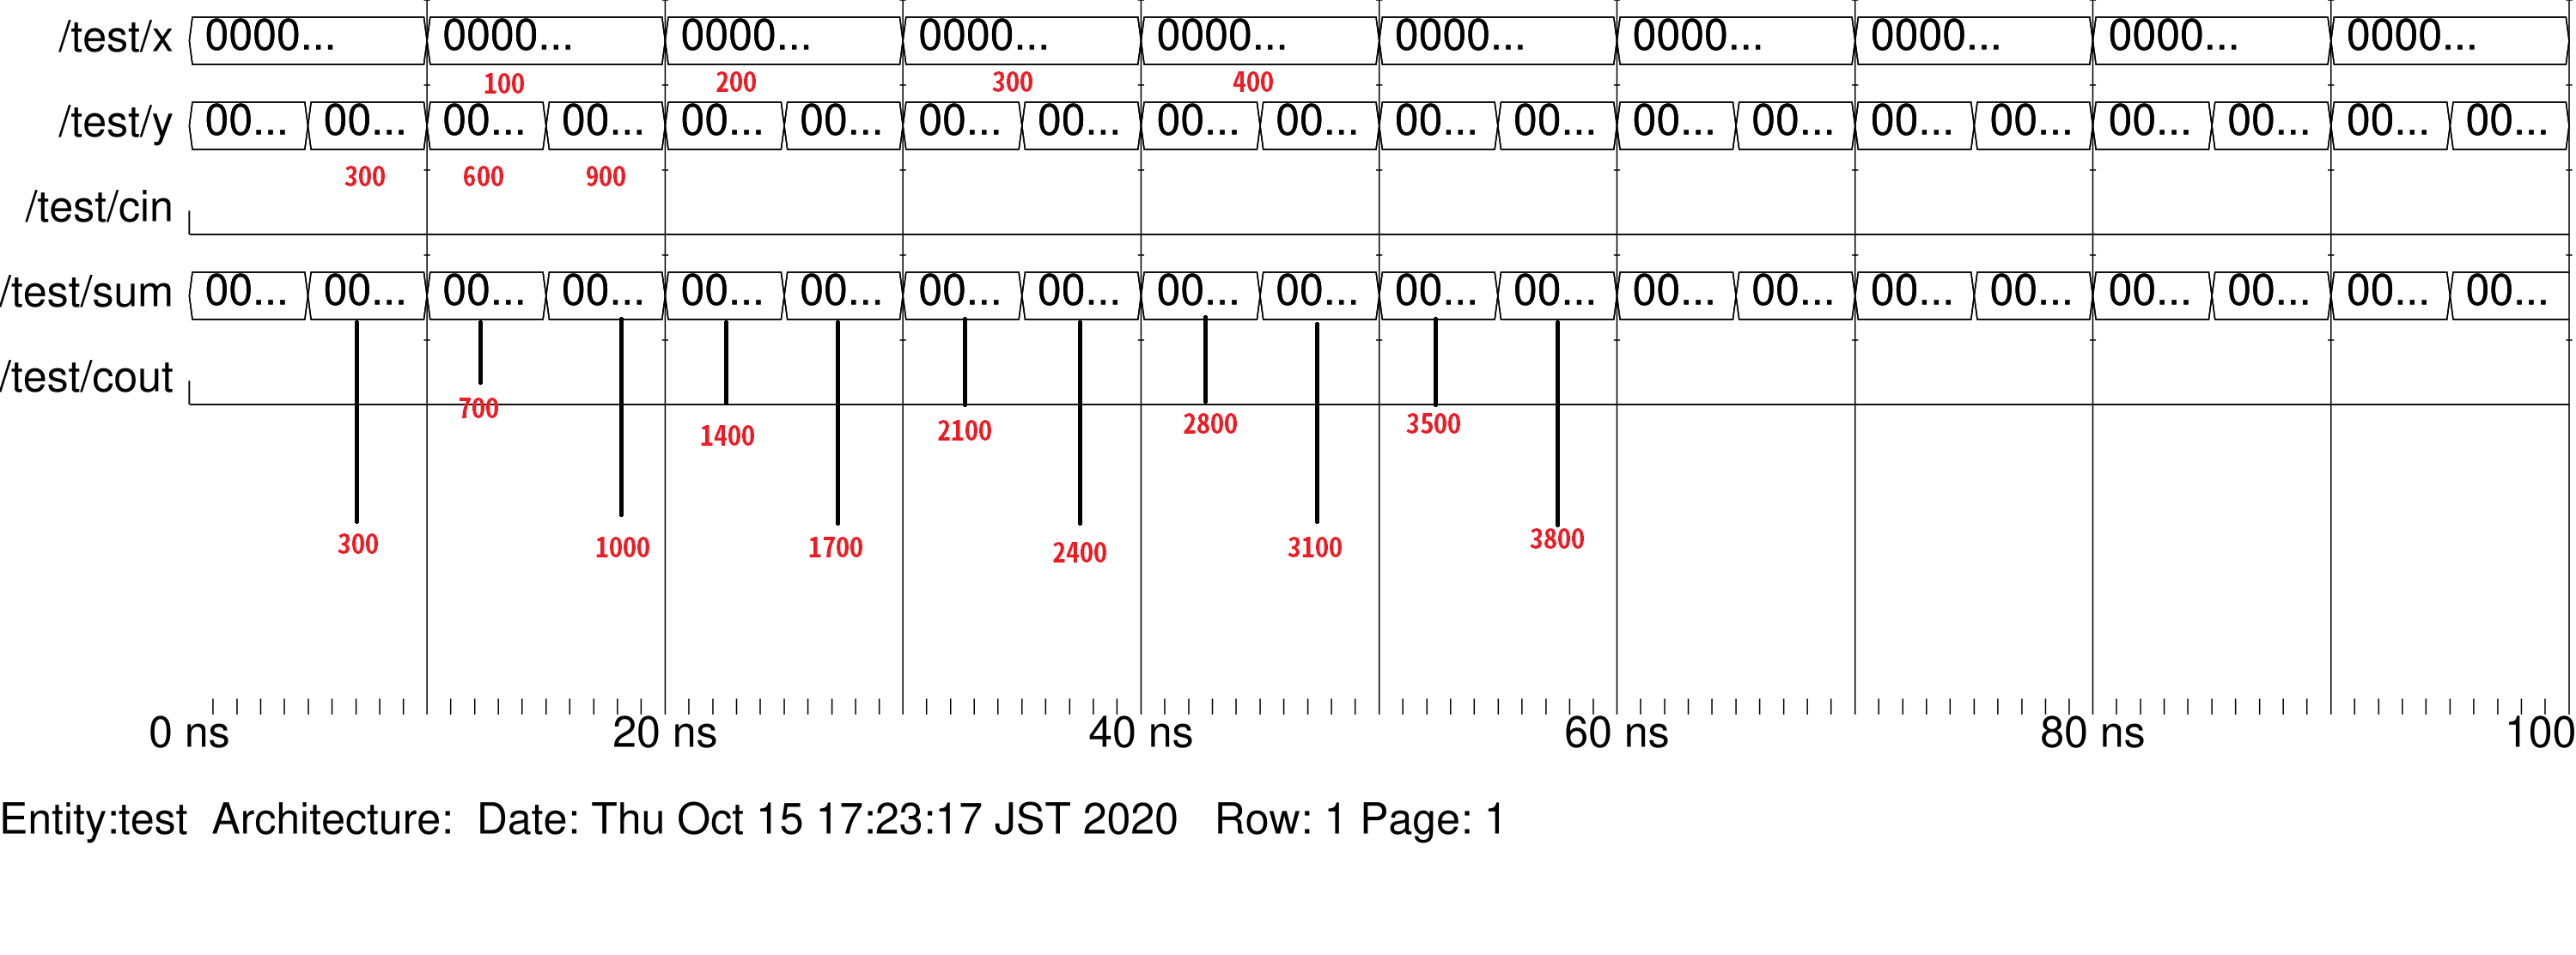
\includegraphics[width=\linewidth]{./src/adder16/adder16_wave21.png}
  \caption{adder16の波形}
\end{figure}

足し算の結果は正しく出力されていることが確認できた。
キャプチャの範囲の外で,coutに桁上げが出力されていることも確認できた。

\subsubsection{論理合成}
論理合成の結果,以下のような回路が作られた。

\begin{figure}[H]
  \centering
  \includegraphics[width=\linewidth]{./src/adder16/adder16_print.png}
  \caption{adder16の回路}
\end{figure}

ロジックエレメント数は19だった。

回路全体の遅延時間は,以下のようになった。

\begin{figure}[H]
  \centering
  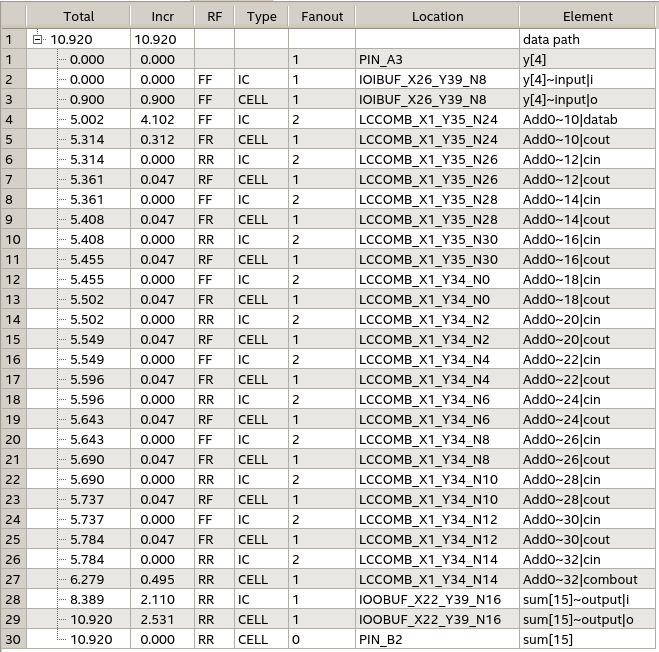
\includegraphics[width=\linewidth]{./src/adder16/adder16Timing.png}
  \caption{adder16の遅延時間}
  \label{adder16の遅延時間}
\end{figure}

\subsection{考察}
\subsubsection{回路のHDL記述}
コード\ref{adder16.v}では,16bitの入出力を定義して,assign句で出力に演算結果を割り当てている。
17bit連接に対して足し算の結果を割り当てているため,結果が16bitに収まらない場合,coutの値は1になる。

コード\ref{testadder16.v}ではテストベンチとして,入力をすべてゼロに初期化し,10nsごとにxを100ずつ加算し,5nsごとにyを300ずつ加算している。

\subsubsection{論理合成}
合成結果より,一桁ごとに桁上りを含めた3入力の全加算器で加算している。
単純な加算機として実装されており,当然桁上りの先読みも行われていないため,そのような記述をすることで,遅延速度が小さくなるのではないかと考える。

遅延時間の表\ref{adder16の遅延時間}より,最長の遅延時間が発生するパスは,最初の全加算器ではなく,(半加算器も含めて)6つめの全加算器への入力から始まっている。
これは,この段階までは配線長とinputIOによる遅延よりも,加算機による遅延のほうが少ないということではないかと予想する。
